\begin{figure}
	\centering
	%\tikzset{external/remake next}
	\begin{tikzpicture}[spy using outlines={rectangle, red, magnification=6,
		size=3.8cm, connect spies}]
		\node{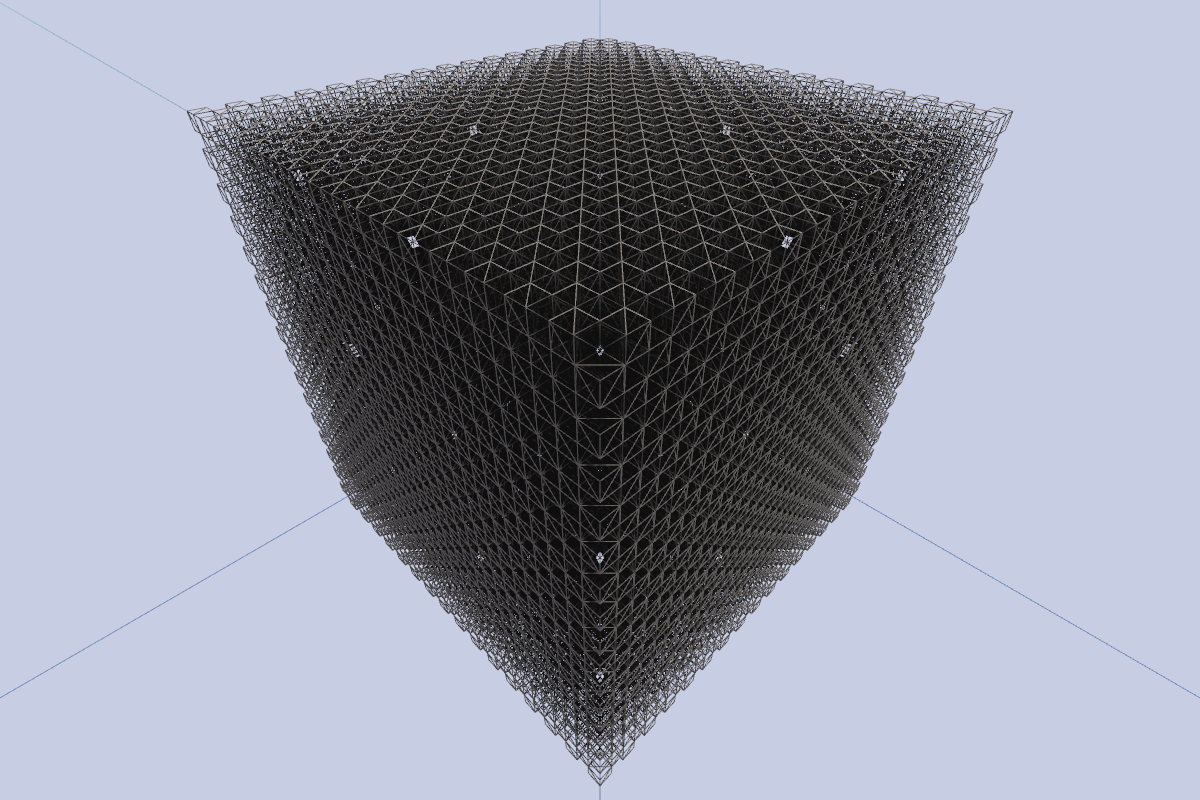
\includegraphics[width=.7\textwidth]{fps-cube.png}};
		\spy on (-3.8,2.65) in node [right] at (-10,2);
		\spy on (0.25,.65) in node [right] at (-10,-2);
	\end{tikzpicture} 
	\caption[Bildschirmfoto der Blockformation in Szenario 2: Halbwürfel.]{Bildschirmfoto der Blockformation in Szenario 2: Halbwürfel. Es wird das Drahtgittermodell der Blöcke dargestellt, um die Menge der angezeigten Elemente zu maximieren. Zur besseren Ansicht sind zwei Bereiche vergrößert dargestellt. Links unten ist die Zerteilung der Würfelseiten in je zwei Dreiecke zu erkennen. Links oben wird ersichtlich, dass das Drahtgittermodell tatsächlich nur die Kanten der Dreiecke zeichnet.}\label{fig:cube}
\end{figure}
Da die Anzahl der zu zeichnenden Objekte in dem ersten Szenario relativ gering ist, wird sie in Szenario 2, welches in Abbildung~\ref{fig:cube} veranschaulicht ist, erhöht. In diesem Szenario wird ein Bereich von $32 \times 32 \times 32$\,Blöcken so befüllt, dass sich an jeder zweiten Stelle ein Block befindet. Zweidimensional entspricht das einem Schachbrettmuster. Die Anzahl der platzierten Blöcke ist damit $\frac{1}{2}\cdot32^3 = 16384$. Die Anzahl der zu zeichnenden Dreiecke beträgt $16384\cdot6 + 5 = 98309$.

In diesem Szenario wird das Drahtgittermodell der Blöcke gezeichnet (das heißt nur die Kanten der zu zeichnenden Dreiecke), weil sonst aufgrund der Anordnung nur wenige Blöcke sichtbar wären. Dennoch kann hier nicht mehr sichergestellt werden, dass auch tatsächlich alle Elemente gezeichnet werden, da selbst mit dem Drahtgittermodell an vielen Stellen Polygone überdeckt werden. Durch die Darstellung als Drahtgittermodell lassen sich nun auch die Kanten der Skybox erkennen. 


\paragraph{\ac{fps}}Der Verlauf der Bildwiederholrate für Szenario 2 ist in Abbildung~\ref{fig:seed-0-cube-fps} dargestellt.
In \sysA{} werden Frames ab Sekunde $11$ erzeugt, in \sysB{} ab Sekunde $13$. Die mittlere Bildwiederholrate in \sysA{} ist \SI{253}{\fps} und in \sysB{} \SI{417}{\fps}. Damit erhöht sich die Bildwiederholrate in \sysB{} um \SI{65}{\percent}. Dieser Wert ist deutlich geringer als in Szenario 1. Dass die Bildwiederholrate in beiden Systemen stark gesunken ist, könnte an einer höheren Last für die \ac{cpu} oder aber für die \ac{gpu} liegen. Die Bildwiederholraten bleiben in beiden Systemen wieder annähernd konstant.
\begin{figure}[!htb]
	\fpsplot{seed-0-cube}
	\caption{Graph des Verlaufs der Bildwiederholrate in Szenario 2: Halbwürfel.}\label{fig:seed-0-cube-fps}
\end{figure}

\paragraph{\ac{cpu}} Die Last der \ac{cpu} in Szenario 2, zu sehen in Abbildung~\ref{fig:seed-0-cube-cpu}, gestaltet sich vergleichbar zu der in Szenario 1. Die Mittelwerte sind mit \SI{13}{\percent} in \sysA{} und \SI{18}{\percent} in \sysB{} nach Rundung identisch zu Szenario 1.
\begin{figure}[!htb]
	\cpuplot{seed-0-cube}
	\caption[Graph des Verlaufs der \glsentryshort{cpu}-Auslastung in Szenario 2: Halbwürfel.]{Graph des Verlaufs der \ac{cpu}-Auslastung in Szenario 2: Halbwürfel.}\label{fig:seed-0-cube-cpu}
\end{figure}
Auffällig ist, dass \sysB{} wie in Szenario 1 in den ersten Sekunden, während des Starts der Blocklib, zwei Auslastungsspitzen besitzt (\SI{32}{\percent} und \SI{50}{\percent}). \sysA{} dagegen besitzt nur eine (\SI{46}{\percent}). Eine mögliche Erklärung dafür ist die Trennung von Simulation und Rendering in verschiedene Threads. Das könnte zu einer zeitweisen Entlastung \ac{cpu} führen, weil die \ac{gpu} Zeit benötigt, um übergebene \glspl{Anweisung} auszuführen, beispielsweise wenn Texturen zum Start auf die \ac{gpu} geladen werden.

\paragraph{\ac{gpu}} Die \ac{gpu}-Last des Halbwürfel-Szenarios unterscheidet sich im Gegensatz zur \ac{cpu}-Auslastung deutlich von der im Hexagon-Szenario gemessenen. In Abbildung~\ref{fig:seed-0-cube-gpu} ist die gemessene \ac{gpu}-Auslastung zeitlich aufgetragen. 
\begin{figure}[!htb]
	\gpuplot{seed-0-cube}
	\caption[Graph des Verlaufs der \glsentryshort{gpu}-Auslastung in Szenario 2: Halbwürfel.]{Graph des Verlaufs der \ac{gpu}-Auslastung in Szenario 2: Halbwürfel.}\label{fig:seed-0-cube-gpu}
\end{figure}

Anders als in Szenario 1 ist in beiden Systemen der Unterschied in der Last unübersehbar. \sysB{} nutzt nach dem Start durchschnittlich \SI{94}{\percent} der Leistung der \ac{gpu}, während \sysA{} nur \SI{60}{\percent} Auslastung erzeugt. Über die gesamte Messdauer liegt \sysB{} damit bei \SI{70}{\percent} Auslastung und \sysA{} bei \SI{45}{\percent}. Betrachtet man nur die Auslastung nach dem Start, lässt sich eine Steigerung der Last um \SI{57}{\percent} errechnen. Die Tatsache, dass die Auslastung der \ac{gpu} in \sysB{} bei knapp \SI{100}{\percent} liegt, bestätigt die Vermutung, dass der niedrige Unterschied der Bildwiederholrate mit der Last für die \ac{gpu} zusammenhängen könnte. In diesem Szenario scheint die Anzahl der generierten Frames in \sysB{} durch die Leistung der \ac{gpu} beschränkt zu sein. 


\paragraph{\ac{ram}} Die Speichernutzung in Szenario 2 wird in Abbildung~\ref{fig:seed-0-cube-mem} gezeigt. Der Ge\-samt-Spei\-cher\-ver\-brauch von \sysA{} steigt im Vergleich zum Hexagon-Szenario leicht, während der Speicherverbrauch von \sysB{} beinahe identisch bleibt. \sysA{} benötigt durchschnittlich \SI{643}{\mega\byte} und \sysB{} \SI{941}{\mega\byte}. Das ist ein Anstieg von \SI{12}{\percent} in \sysA{} und eine leichte Verringerung um \SI{1}{\percent} in \sysB{} gegenüber dem letzten Szenario. Weiterhin zeigt \sysB{} einen großen Speicherverbrauch während des Starts der Blocklib (\SI{1732}{\mega\byte}).

\begin{figure}[!htb]
	\memplot[xticklabels={,,},xlabel={}]{seed-0-cube-single-mem.csv}{\sysA{}}
	\\\memplot{seed-0-cube-multi-mem.csv}{\sysB{}}
	\caption{Graph des Verlaufs der Speichernutzung in Szenario 2: Halbwürfel.}\label{fig:seed-0-cube-mem}
\end{figure} 

Die Speichernutzung der kurzlebigen Objekte ist sowohl in \sysA{} mit \SI{53}{\mega\byte\per\second} als auch in \sysB{} mit \SI{101}{\mega\byte\per\second} niedriger als in Szenario 1. Insbesondere \sysB{} verbraucht mit neu erzeugten Objekten weniger als halb so viel Speicher. Vergleicht man die beiden Systeme in diesem Szenario, erhält man einen Anstieg von \SI{91}{\percent} Speicherverbrauch mit \sysB{}. Der geringere Speicherverbrauch führt auch zu einer geringeren Anzahl an Garbage-Collections. Die Anzahl der Garbage-Collections im gemessenen Zeitraum in \sysB{} mit 10 Collections ist um eine niedriger als in \sysA{}. Der zusätzliche Speicher gleicht also den höheren dauerhaften Speicherverbrauch aus. 

Der langlebige Speicherverbrauch bleibt in beiden Systemen mit \SI{296}{\mega\byte} (\sysA{}) und \SI{320}{\mega\byte} (\sysB{}) sehr konstant. In \sysA{} sinkt der Speicherverbrauch, wie auch schon im Hexagon-Szenario zu beobachten, nach etwa 45 Sekunden auf zum Ende nur noch \SI{129}{\mega\byte}.